%%% LaTeX Template: Article/Thesis/etc. with colored headings and special fonts
%%%
%%% Source: http://www.howtotex.com/
%%% Feel free to distribute this template, but please keep to referal to http://www.howtotex.com/ here.
%%% February 2011
%%%
%%% Modified January 2016 by CDM

%%%  Preamble
\documentclass[11pt,letterpaper]{article}
\usepackage[margin=1.0in]{geometry}
\usepackage[T1]{fontenc}
\usepackage[bitstream-charter]{mathdesign}
\usepackage[latin1]{inputenc}					
\usepackage{amsmath}						
\usepackage{xcolor}
\usepackage{cite}
\usepackage{hyphenat}
\usepackage{graphicx}
\usepackage{float}
\usepackage{subfigure}
\usepackage{sectsty}
\usepackage[compact]{titlesec} 
\usepackage[tablegrid]{vhistory}
\usepackage{pbox}
\allsectionsfont{\color{accentcolor}\scshape\selectfont}

%%% Definitions
%%%%%%%%%%%%%%%%%%%%%%%%%%%%%%%%%%%%%%%%%%%%%%%%%%%%
% UPDATE THIS SECTION TO YOUR TEAM AND SEMESTER INFO
\definecolor{accentcolor}{rgb}{0.0,0.0,0.5} 
\newcommand{\teamname}{Runtime Terror}
\newcommand{\productname}{Turing Board}
\newcommand{\coursename}{CSE 4317: Senior Design II}
\newcommand{\semester}{Spring 2022}
\newcommand{\docname}{Detailed Design Specification}
\newcommand{\department}{Department of Computer Science \& Engineering}
\newcommand{\university}{The University of Texas at Arlington}
\newcommand{\authors}{Sahaj Amatya \\ Sarker Nadir Afridi Azmi \\ Kendall Buchanan \\ Keaton Koehler \\ Happy Ndikumnaa \\ Lydia Sarver}

%%% Headers and footers
\usepackage{fancyhdr}
	\pagestyle{fancy}						% Enabling the custom headers/footers
\usepackage{lastpage}	
	% Header (empty)
	\lhead{}
	\chead{}
	\rhead{}
	% Footer
	\lfoot{\footnotesize \teamname \ - \semester}
	\cfoot{}
	\rfoot{\footnotesize page \thepage\ of \pageref{LastPage}}	% "Page 1 of 2"
	\renewcommand{\headrulewidth}{0.0pt}
	\renewcommand{\footrulewidth}{0.4pt}

%%% Change the abstract environment
\usepackage[runin]{abstract}			% runin option for a run-in title
%\setlength\absleftindent{30pt}			% left margin
%\setlength\absrightindent{30pt}		% right margin
\abslabeldelim{\quad}	
\setlength{\abstitleskip}{-10pt}
\renewcommand{\abstractname}{}
\renewcommand{\abstracttextfont}{\color{accentcolor} \small \slshape}	% slanted text

%%% Start of the document
\begin{document}

%%% Cover sheet
%%%%%%%%%%%%%%%%%%%%%%%%%%%%%%%%%%%%%%%%%%%%%%%%%%%%%%%%%%%%%%%%%%%%%%%%%%%%
%   CHANGE THE GRAPHIC HERE. PUT YOUR IMAGE IN THE 'images' 
%   FOLDER AND UPDATE THE NAME FROM 'images/test_image' TO YOUR IMAGE NAME
{\centering \huge \color{accentcolor} \sc \textbf{\department \\ \university} \par}
\vspace{0.5 in}
{\centering \huge \color{accentcolor} \sc \textbf{\docname \\ \coursename \\ \semester} \par}
\vspace{0.3 in}
\begin{figure}[h!]
	\centering
   	
\includegraphics[width=0.60\textwidth]{images/turing_logo} 
\end{figure}
\vspace{0.2 in}
{\centering \huge \color{accentcolor} \sc \textbf{\teamname \\ \productname} \par}
\vspace{0.3 in}
{\centering \large \sc \textbf{\authors} \par}
\newpage


%\vspace{1 in}
%\centerline{January 13th, 2012}
%\newpage

%%% Revision History
%%%%%%%%%%%%%%%%%%%%%%%%%%%%%%%%%%%%%%%%%%%%%%%%%%%%%%%%%%%%%%%%%
%   EACH '\vhEntry' BEGINS A ROW; EACH {} IS A COLUMN. UPDATE
%   THIS TO REFLECT YOUR REVISION HISTORY
\begin{versionhistory}
  	\vhEntry{0.1}{1.01.2016}{GH}{document creation}
  	\vhEntry{0.2}{1.05.2016}{AT|GH}{complete draft}
  	\vhEntry{0.3}{1.12.2016}{AT|GH}{release candidate 1}
  	\vhEntry{1.0}{1.20.2016}{AT|GH|CB}{official release}
  	\vhEntry{1.1}{1.31.2016}{AL}{added design review requests}
\end{versionhistory}
\newpage

%%% Table of contents
\setcounter{tocdepth}{2}
\tableofcontents
\newpage

%%% List of figures and tables (optional)
\listoffigures
\listoftables
\newpage

%%% Document sections
%%%%%%%%%%%%%%%%%%%%%%%%%%%%%%%%%%%%%%%%%%%%%%%%%%%%%%%%%%%%%%%
%   THIS IMPORTS LATEX FILES FROM THE TEX FOLDER. COPY/PASTE TO
%   ADD SECTIONS AS NEEDED AND CREATE FILE FOR IT IN TEX FOLDER
\section{Introduction}
Your introduction should provide a brief overview of the product concept and a reference to the requirement specification and architectural design documents in 1 or 2 paragraphs. The purpose is to provide the reader with the location of relevant background material that lead to the design details presented in this document.

\section{System Overview}
The main controls layer is in charge of processing and sending out the majority of the signals on the Turing Board. It uses the Jetson TX2 to communicate with the microprocessor in the wheels and turning layer to control the wheels and turning mechanism. There are several sensors in the wheels and turning layer that send information via the microprocessor to the Jetson as inputs. The Jetson also receives inputs from the power layer to know how much power is left in the battery. The last input to the Jetson comes from the Human Machine Interface (HMI) layer. This layer consists of items used to allow the Turing Board to understand the world around it and operate more appropriately. Along with the human machine interface layer, the computer vision layer also contributes to the Jetson TX2 receiving feedback from its environment. The computer vision layer uses RGB imagery and stereo and infrared imagery to see obstacles and the user depending on the mode it is currently in. Finally, the remote control for the Turing Board allows the user to control the board as an electric longboard when in the respective mode. The app boasts many features including user authentication and ride data analysis.

%%%%%%%%%%%%%%%%%%%%%%%%%%%%%%%%%%%%%%%%%%%%%%%%%%%%%%%%%%%%%%%%%%%%%%%%%%%%%%%%%%%%%%%%%%%%%
% If you want to change the image, put your image in the images folder and change "data_flow" 
% to the name of your image. You can also change the caption (System architecture) to 
% something else if you want.
\begin{figure}[h!]
	\centering
 	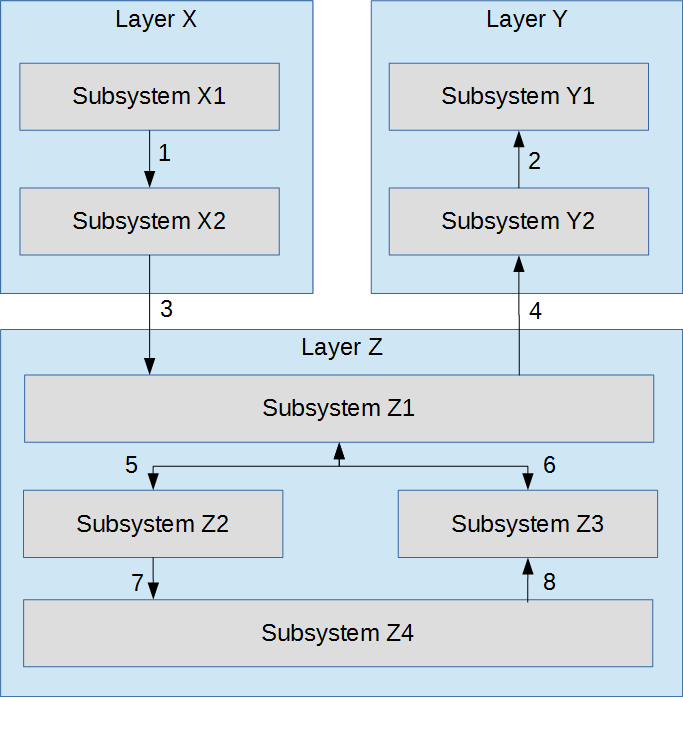
\includegraphics[width=0.90\textwidth]{images/data_flow} % Change me
 \caption{System Architecture}
\end{figure}

\newpage
%\section{Subsystem Definitions \& Data Flow}
%This section breaks down your layer abstraction to another level of detail. Here you grapically represent the logical subsytems that compose each layer and show the interactions/interfaces between those subsystems. A subsystem can be thought of as a programming unit that implements one of the major functions of the layer. It, therefore, has data elements that serve as source/sinks for other subsystems. The logical data elements that flow between subsystems need to be explicitly defined at this point, beginning with a data flow-like diagram based on the block diagram.

%%%%%%%%%%%%%%%%%%%%%%%%%%%%%%%%%%%%%%%%%%%%%%%%%%%%%%%%%%
%  BE SURE TO UPDATE THE IMAGE CAPTION
\begin{figure}[h!]
	\centering
 	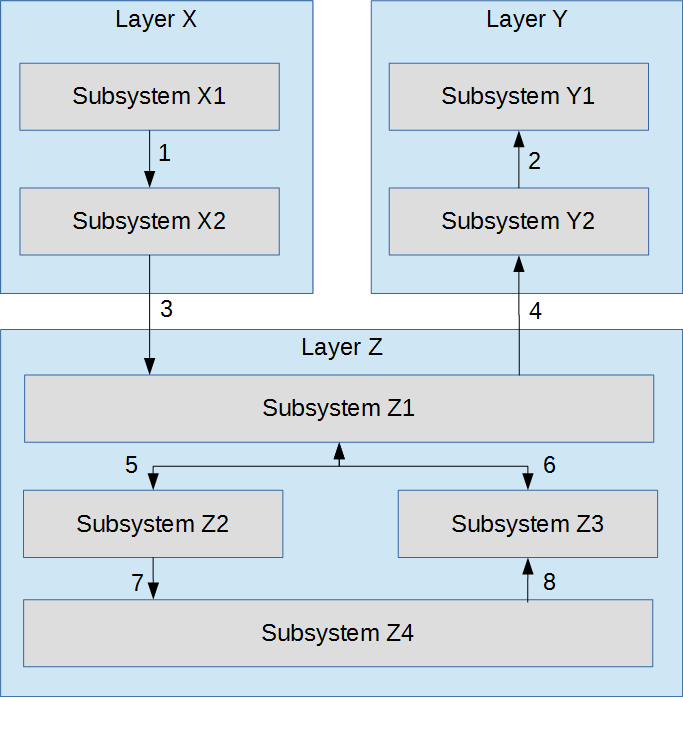
\includegraphics[width=\textwidth]{images/data_flow} % Image
 \caption{A simple data flow diagram} % Caption
\end{figure}

\newpage
\section{Power Layer Subsystems}
Each electrical component has a specific power requirement and this layer is responsible for providing that power.

\subsection{Layer Hardware}
The Turing Board includes an ER 36 volt battery and Songhe LM2596S Buck Converters. 

\subsection{Layer Operating System}
No operating system is used in this layer.

\subsection{Layer Software Dependencies}
No software is used in this layer.

\subsection{Subsystem 1}
This module consists of a Li-Po battery which provides power to a Buck Converter. It is an ER 36 volt battery with a 30A current output.

%%%%%%%%%%%%%%%%%%%%%%%%%%%%%%%%%%%%%%%%%%%%%%%%%%%%%%%%%%
%  BE SURE TO UPDATE THE IMAGE CAPTION
\begin{figure}[h!]
	\centering
 	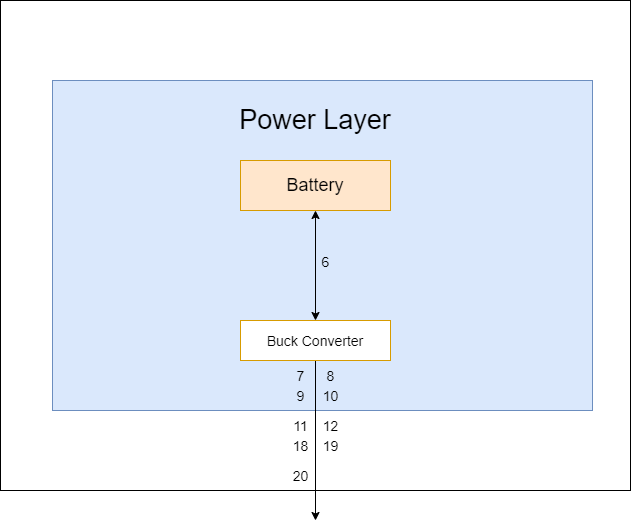
\includegraphics[width=0.60\textwidth]{images/Bat.png} % Image
 \caption{Battery Subsystem in Power Layer} % Caption
\end{figure}

\subsubsection{Subsystem Hardware}
The battery outputs around 36 volts rated at 8000mAh.

\subsubsection{Subsystem Operating System}
No operating system is used in this subsystem.

\subsubsection{Subsystem Software Dependencies}
No software is used in this subsystem

\subsubsection{Subsystem Programming Languages}
No programming languages are used in this subsystem.

\subsubsection{Subsystem Data Structures}
No data structures are used in this subsystem.

\subsubsection{Subsystem Data Processing}
No algorithms are used in this subsystem.

\subsection{Subsystem 2}
The entire module consists of a Li-Po battery to provide power to a Buck Converter which then powers the rest of the system. 

%%%%%%%%%%%%%%%%%%%%%%%%%%%%%%%%%%%%%%%%%%%%%%%%%%%%%%%%%%
%  BE SURE TO UPDATE THE IMAGE CAPTION
\begin{figure}[h!]
	\centering
 	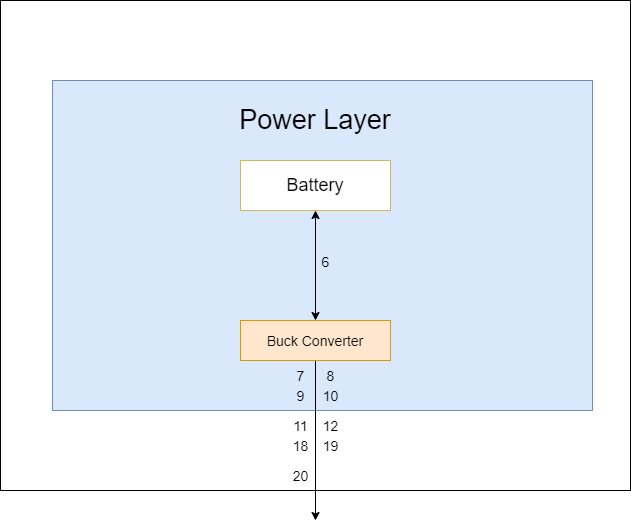
\includegraphics[width=0.60\textwidth]{images/Buck.png} % Image
 \caption{Buck Converter Subsystem in Power Layer} % Caption
\end{figure}

\subsubsection{Subsystem Hardware}
With an input voltage of 36 volts from the battery, the buck converters are able to output between 1.25V \textasciitilde 34V continuously.

\subsubsection{Subsystem Operating System}
No operating system is used in this subsystem.

\subsubsection{Subsystem Software Dependencies}
No software is used in this subsystem

\subsubsection{Subsystem Programming Languages}
No programming languages are used in this subsystem.

\subsubsection{Subsystem Data Structures}
No data structures are used in this subsystem.

\subsubsection{Subsystem Data Processing}
No algorithms are used in this subsystem.

\newpage
\section{Controls Software Layer Subsystems}
The controls layer is responsible for binding all modules of the Turing Board to be part of the same system. All data coming in is intercepted by this layer and forwarded to the respective modules which are responsible for processing the forwarded data.

\subsection{Layer Hardware}
The hardware involved in this layer consists of the following:
\begin{itemize}
    \item Nvidia Jetson TX2 responsible for running the controls code.
    \item VESC responsible for the speed control of the wheels.
    \item Intel real sense camera responsible for capturing real time footage for the follow-me feature and autonomous navigation.
    \item Texas Instruments Tiva C Series microcontroller which controls the turning mechanism.
\end{itemize}

\subsection{Layer Operating System}
The Layer makes use of the Linux operating system to run applications such as the control code.

\subsection{Layer Software Dependencies}
\begin{itemize}
    \item Python Dependencies
    \begin{itemize}
        \item PyVESC
        \item Pyrebase
        \item Pyserial
        \item Pycrc
        \item Threading
    \end{itemize}
\end{itemize}

\subsection{Controls Subsystem}
There are three main components of project which calls for this piece of software which must all be non-blocking in nature to ensure the entire system stays responsive.
\begin{itemize}
    \item Reading data from the microcontroller.
    \item Forwarding data to the microcontroller.
    \item Fetching data from the Firebase Real-time database.
\end{itemize}

\begin{figure}[h!]
	\centering
 	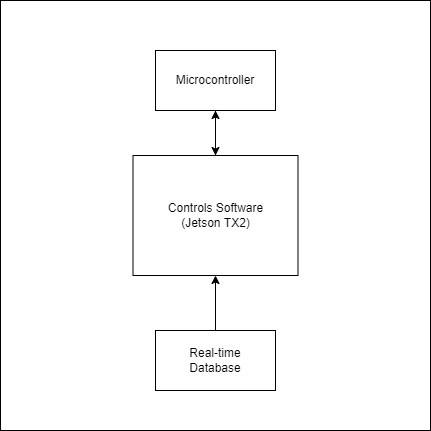
\includegraphics[width=0.60\textwidth]{images/Controls Software Subsystem.drawio.png}
 \caption{Example subsystem description diagram}
\end{figure}

\subsubsection{Subsystem Hardware}
The controls subsystem does not consist of explicit hardware. All work is done through software to communicate information.

\subsubsection{Subsystem Operating System}
The controls subsystem does not make use of an underlying operating system. The layer makes use of the Linux operating system.

\subsubsection{Subsystem Software Dependencies}
\begin{itemize}
    \item Python Dependencies
    \begin{itemize}
        \item PyVESC
        \item Pyrebase
        \item Pyserial
        \item Pycrc
        \item Threading
    \end{itemize}
\end{itemize}

\subsubsection{Subsystem Programming Languages}
\begin{itemize}
    \item Python
    \begin{itemize}
        \item Used for the main controls system.
    \end{itemize}
    \item C
    \begin{itemize}
        \item Used to program the microcontroller.
    \end{itemize}
\end{itemize}

\subsubsection{Subsystem Data Structures}
\begin{itemize}
    \item Classes
    \begin{itemize}
        \item Controls
        \begin{itemize}
            \item Responsible for running the controls code.
        \end{itemize}
        \item SerialCommunication
        \begin{itemize}
            \item Establishes connection with the microcontroller.
        \end{itemize}
    \end{itemize}
\end{itemize}

\subsubsection{Subsystem Data Processing}
After fetching data from the database, the controls software will process the data first to an extent. Since data coming in will be floating point values, it first needs to be translated into value which the microcontroller can understand. So, the entire range of data from the remote control app is taken and the required data is mapped from 0-255 which is then forwarded to the microcontroller which causes the wheels to change speed. As part of the same data packet, angle data from the controls code is also sent to the microcontroller which aids in turning the turning mechanism to a specific angle with respect to the turning mechanisms origin. Any data such as weight values if someone is standing on the long board (an integral part of the design so that the software knows when to turn off the turning mechanism) is received back in the same data format (0-255) which gets translated to weight values inside of the controls code.
\newpage
\section{HMI Layer Subsystems}
This layer involves the various sensors and indicators that interact between the Turing Board and the user directly. This includes a load cell or force-sensing resistor for a weight sensor, a piezoelectric speaker, a printed ArUco symbol, a PWM-capable LED strip, a Tiva C Series Microcontroller, and various electrical components. The weight sensor, speaker, and LEDs communicate directly with the Tiva C Series, while the ArUco symbol is recognized by an Intel RealSense camera which sends the data to the Jetson TX2 via the CV Layer. The Tiva C Series is programmed using C and Assembly via Code Composer Studio 10, while the libraries used for the CV layer mainly use C++ and a generic IDE. This is capable of running on both Windows, MacOS, and Linux.

\subsection{Layer Hardware}
This layer uses a generic piezoelectric speaker (buzzer), a load cell or force-sensing resistor (weight sensor), a printed ArUco symbol generated online (follow anklet), a strip of PWM-capable LEDs approximately 10ft in length, a Tiva C Series, and various electrical components (MOSFETs, resistors, ADC, etc.).

\subsection{Layer Operating System}
N/A.

\subsection{Layer Software Dependencies}
This layer depends on code done in Code Composer Studio (v10.2) to program the Tiva C Series and drive the various HMI subsystems. We also used the site https://chev.me/arucogen/ to generate our ArUco symbol.

\subsection{Weight Sensor}
The weight sensor will be implemented as a safety feature primarily, with future uses in load carrying. When a user is riding on the board, it will detect if they fall off to initiate an emergency stop. When a user attempts to get on the board while in autonomous mode it will trigger an alert noise to notify the user it is not safe to ride.

\begin{figure}[h!]
	\centering
 	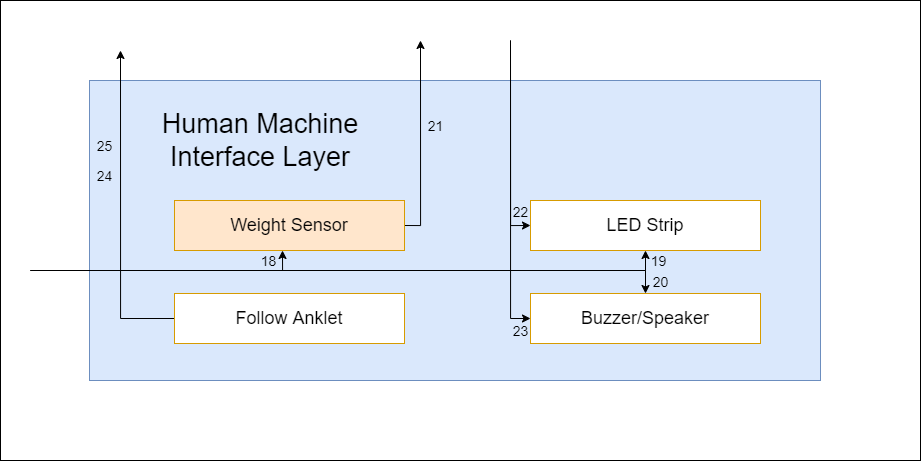
\includegraphics[width=0.60\textwidth]{images/Kendall/Weight Sensor.png}
 \caption{Weight Sensor Subsystem in HMI Layer}
\end{figure}

\subsubsection{Subsystem Hardware}
The weight sensor will implement either a generic load cell or force-sensing resistor in or order to determine the weight/pressure being generated by an item/person placed on top. This will detect and send any weight data to a Tiva C Series to parse and decode.

\subsubsection{Subsystem Operating System}
N/A.

\subsubsection{Subsystem Software Dependencies}
The weight sensor requires the Tiva C Series to read and parse any data. This, in turn, requires Code Composer Studio 10 to create code to parse/read the data and program the Tiva accordingly.

\subsubsection{Subsystem Programming Languages}
Code Composer Studio 10 has code written in C and Assembly.

\subsubsection{Subsystem Data Structures}
The data read in by the sensor is formed into 24-bit "packets" sent along a datastream to the Tiva running at 100kHz. This is done by transmitting one bit per clock using an ADC. This data, which correspond with an external linear force, is then read and parsed by the Tiva and any relevant data is passed to the other subsystems (LEDs and Buzzer/Speaker) to alert of a weight change.

\subsubsection{Subsystem Data Processing}
N/A.

\subsection{Buzzer/Speaker}
The buzzer/speaker will be used to alert the user if they attempt to step on the board when it is in an autonomous mode. When the weight sensor detects a person attempting to stand on the board when in autonomous mode, the buzzer will begin to sound an alert to notify the user it is unsafe to stand on it.

\begin{figure}[h!]
	\centering
 	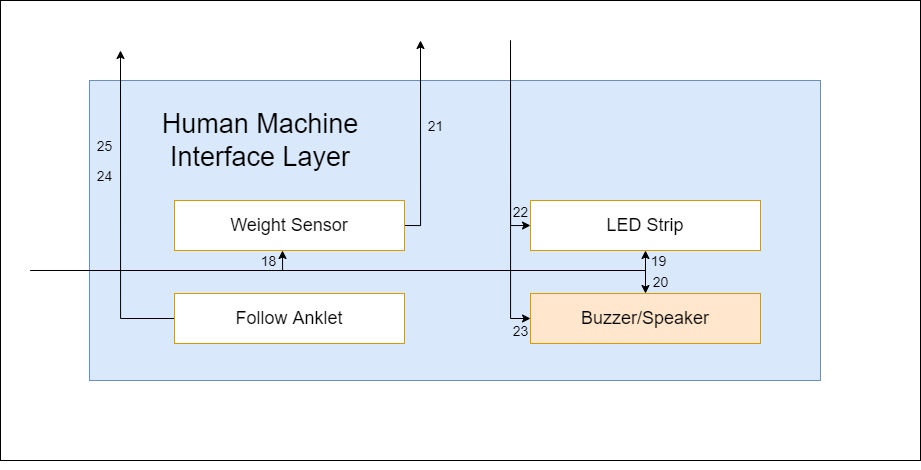
\includegraphics[width=0.60\textwidth]{images/Kendall/Buzzer.png}
 \caption{Buzzer/Speaker Subsystem in HMI Layer}
\end{figure}

\subsubsection{Subsystem Hardware}
This subsystem uses a generic piezoelectric speaker powered and run by a Tiva C Series to emit a sound as an alert on various conditions.

\subsubsection{Subsystem Operating System}
N/A.

\subsubsection{Subsystem Software Dependencies}
Code Composer Studio 10 is used to send signals to the piezoelectric speaker in order to emit a sound of a pre-determined frequency and length.

\subsubsection{Subsystem Programming Languages}
Code Composer Studio 10 has code written in C and Assembly.

\subsubsection{Subsystem Data Structures}
A signal is sent from the Tiva to the speaker using a 32-bit value to determine the frequency at which to emit the sound. The Tiva also uses a 32-bit variable to determine how long to emit the signal for before sending a stop command.

\subsubsection{Subsystem Data Processing}
N/A.

\subsection{LED Strip}
The LED strip will be used to indicate to the user what mode the Turing Board is currently in. These modes will be differentiated by implementing a different color for each mode. 

\begin{figure}[h!]
	\centering
 	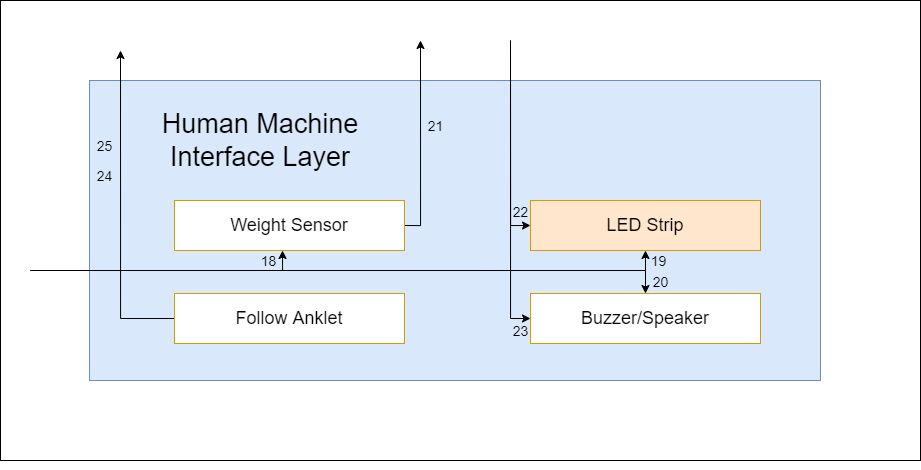
\includegraphics[width=0.60\textwidth]{images/Kendall/LED Strip.png}
 \caption{LED Strip Subsystem in HMI Layer}
\end{figure}

\subsubsection{Subsystem Hardware}
These LEDs are specifically PWM-capable and rated at up to 12V. It also implements a Tiva C Series to control the LEDs.

\subsubsection{Subsystem Operating System}
N/A.

\subsubsection{Subsystem Software Dependencies}
The LEDs are powered and controlled by the Tiva using Code Composer Studio.

\subsubsection{Subsystem Programming Languages}
Code Composer Studio 10 has code written in C and Assembly.

\subsubsection{Subsystem Data Structures}
The LEDs are each fed a 256-bit value corresponding to the Red, Blue, and Green data lines from the Tiva. This, in turn, activates the respective LED color to create various combinations based on each R/G/B input values.

\subsubsection{Subsystem Data Processing}
N/A.

\subsection{Follow Anklet}
The Anklet will be a worn feature used for the CV to track and follow the rider in follow-along mode.

\begin{figure}[h!]
	\centering
 	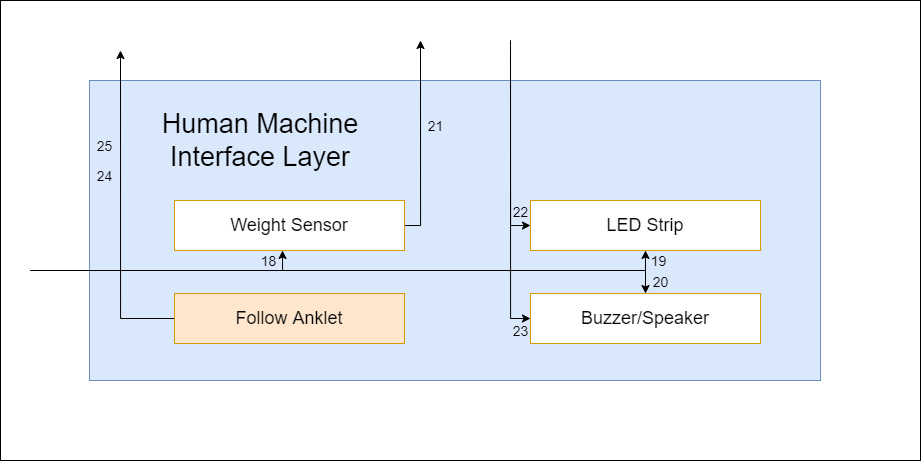
\includegraphics[width=0.60\textwidth]{images/Kendall/Anklet.png}
 \caption{Follow Anklet Subsystem in HMI Layer}
\end{figure}

\subsubsection{Subsystem Hardware}
This subsystem simply uses an ArUco symbol printed out on a strip of paper long enough to wrap around one's ankle.

\subsubsection{Subsystem Operating System}
N/A.

\subsubsection{Subsystem Software Dependencies}
This depends on the ArUco library based on the OpenCV library used to detect and track a generated symbol.

\subsubsection{Subsystem Programming Languages}
This uses C/C++ in the provided libraries required to detect and track the symbol.

\subsubsection{Subsystem Data Structures}
N/A.

\subsubsection{Subsystem Data Processing}
Uses an algorithm defined in the ArUco/OpenCV libraries to recognize and track the generated symbol.
\newpage
\section{Appendix A}
Include any additional documents (CAD design, circuit schematics, etc) as an appendix as necessary.
\newpage

%%% References
\bibliographystyle{plain}
\bibliographystyle{reference/IEEEtran_custom}
\bibliography{reference/refs}{}

\end{document}